% Options for packages loaded elsewhere
\PassOptionsToPackage{unicode}{hyperref}
\PassOptionsToPackage{hyphens}{url}
%
\documentclass[
  10pt,
]{article}
\usepackage{amsmath,amssymb}
\usepackage{iftex}
\ifPDFTeX
  \usepackage[T1]{fontenc}
  \usepackage[utf8]{inputenc}
  \usepackage{textcomp} % provide euro and other symbols
\else % if luatex or xetex
  \usepackage{unicode-math} % this also loads fontspec
  \defaultfontfeatures{Scale=MatchLowercase}
  \defaultfontfeatures[\rmfamily]{Ligatures=TeX,Scale=1}
\fi
\usepackage{lmodern}
\ifPDFTeX\else
  % xetex/luatex font selection
\fi
% Use upquote if available, for straight quotes in verbatim environments
\IfFileExists{upquote.sty}{\usepackage{upquote}}{}
\IfFileExists{microtype.sty}{% use microtype if available
  \usepackage[]{microtype}
  \UseMicrotypeSet[protrusion]{basicmath} % disable protrusion for tt fonts
}{}
\makeatletter
\@ifundefined{KOMAClassName}{% if non-KOMA class
  \IfFileExists{parskip.sty}{%
    \usepackage{parskip}
  }{% else
    \setlength{\parindent}{0pt}
    \setlength{\parskip}{6pt plus 2pt minus 1pt}}
}{% if KOMA class
  \KOMAoptions{parskip=half}}
\makeatother
\usepackage{xcolor}
\usepackage[margin=0.5in]{geometry}
\usepackage{color}
\usepackage{fancyvrb}
\newcommand{\VerbBar}{|}
\newcommand{\VERB}{\Verb[commandchars=\\\{\}]}
\DefineVerbatimEnvironment{Highlighting}{Verbatim}{commandchars=\\\{\}}
% Add ',fontsize=\small' for more characters per line
\usepackage{framed}
\definecolor{shadecolor}{RGB}{248,248,248}
\newenvironment{Shaded}{\begin{snugshade}}{\end{snugshade}}
\newcommand{\AlertTok}[1]{\textcolor[rgb]{0.94,0.16,0.16}{#1}}
\newcommand{\AnnotationTok}[1]{\textcolor[rgb]{0.56,0.35,0.01}{\textbf{\textit{#1}}}}
\newcommand{\AttributeTok}[1]{\textcolor[rgb]{0.13,0.29,0.53}{#1}}
\newcommand{\BaseNTok}[1]{\textcolor[rgb]{0.00,0.00,0.81}{#1}}
\newcommand{\BuiltInTok}[1]{#1}
\newcommand{\CharTok}[1]{\textcolor[rgb]{0.31,0.60,0.02}{#1}}
\newcommand{\CommentTok}[1]{\textcolor[rgb]{0.56,0.35,0.01}{\textit{#1}}}
\newcommand{\CommentVarTok}[1]{\textcolor[rgb]{0.56,0.35,0.01}{\textbf{\textit{#1}}}}
\newcommand{\ConstantTok}[1]{\textcolor[rgb]{0.56,0.35,0.01}{#1}}
\newcommand{\ControlFlowTok}[1]{\textcolor[rgb]{0.13,0.29,0.53}{\textbf{#1}}}
\newcommand{\DataTypeTok}[1]{\textcolor[rgb]{0.13,0.29,0.53}{#1}}
\newcommand{\DecValTok}[1]{\textcolor[rgb]{0.00,0.00,0.81}{#1}}
\newcommand{\DocumentationTok}[1]{\textcolor[rgb]{0.56,0.35,0.01}{\textbf{\textit{#1}}}}
\newcommand{\ErrorTok}[1]{\textcolor[rgb]{0.64,0.00,0.00}{\textbf{#1}}}
\newcommand{\ExtensionTok}[1]{#1}
\newcommand{\FloatTok}[1]{\textcolor[rgb]{0.00,0.00,0.81}{#1}}
\newcommand{\FunctionTok}[1]{\textcolor[rgb]{0.13,0.29,0.53}{\textbf{#1}}}
\newcommand{\ImportTok}[1]{#1}
\newcommand{\InformationTok}[1]{\textcolor[rgb]{0.56,0.35,0.01}{\textbf{\textit{#1}}}}
\newcommand{\KeywordTok}[1]{\textcolor[rgb]{0.13,0.29,0.53}{\textbf{#1}}}
\newcommand{\NormalTok}[1]{#1}
\newcommand{\OperatorTok}[1]{\textcolor[rgb]{0.81,0.36,0.00}{\textbf{#1}}}
\newcommand{\OtherTok}[1]{\textcolor[rgb]{0.56,0.35,0.01}{#1}}
\newcommand{\PreprocessorTok}[1]{\textcolor[rgb]{0.56,0.35,0.01}{\textit{#1}}}
\newcommand{\RegionMarkerTok}[1]{#1}
\newcommand{\SpecialCharTok}[1]{\textcolor[rgb]{0.81,0.36,0.00}{\textbf{#1}}}
\newcommand{\SpecialStringTok}[1]{\textcolor[rgb]{0.31,0.60,0.02}{#1}}
\newcommand{\StringTok}[1]{\textcolor[rgb]{0.31,0.60,0.02}{#1}}
\newcommand{\VariableTok}[1]{\textcolor[rgb]{0.00,0.00,0.00}{#1}}
\newcommand{\VerbatimStringTok}[1]{\textcolor[rgb]{0.31,0.60,0.02}{#1}}
\newcommand{\WarningTok}[1]{\textcolor[rgb]{0.56,0.35,0.01}{\textbf{\textit{#1}}}}
\usepackage{longtable,booktabs,array}
\usepackage{calc} % for calculating minipage widths
% Correct order of tables after \paragraph or \subparagraph
\usepackage{etoolbox}
\makeatletter
\patchcmd\longtable{\par}{\if@noskipsec\mbox{}\fi\par}{}{}
\makeatother
% Allow footnotes in longtable head/foot
\IfFileExists{footnotehyper.sty}{\usepackage{footnotehyper}}{\usepackage{footnote}}
\makesavenoteenv{longtable}
\usepackage{graphicx}
\makeatletter
\def\maxwidth{\ifdim\Gin@nat@width>\linewidth\linewidth\else\Gin@nat@width\fi}
\def\maxheight{\ifdim\Gin@nat@height>\textheight\textheight\else\Gin@nat@height\fi}
\makeatother
% Scale images if necessary, so that they will not overflow the page
% margins by default, and it is still possible to overwrite the defaults
% using explicit options in \includegraphics[width, height, ...]{}
\setkeys{Gin}{width=\maxwidth,height=\maxheight,keepaspectratio}
% Set default figure placement to htbp
\makeatletter
\def\fps@figure{htbp}
\makeatother
\setlength{\emergencystretch}{3em} % prevent overfull lines
\providecommand{\tightlist}{%
  \setlength{\itemsep}{0pt}\setlength{\parskip}{0pt}}
\setcounter{secnumdepth}{-\maxdimen} % remove section numbering
\newlength{\cslhangindent}
\setlength{\cslhangindent}{1.5em}
\newlength{\csllabelwidth}
\setlength{\csllabelwidth}{3em}
\newlength{\cslentryspacingunit} % times entry-spacing
\setlength{\cslentryspacingunit}{\parskip}
\newenvironment{CSLReferences}[2] % #1 hanging-ident, #2 entry spacing
 {% don't indent paragraphs
  \setlength{\parindent}{0pt}
  % turn on hanging indent if param 1 is 1
  \ifodd #1
  \let\oldpar\par
  \def\par{\hangindent=\cslhangindent\oldpar}
  \fi
  % set entry spacing
  \setlength{\parskip}{#2\cslentryspacingunit}
 }%
 {}
\usepackage{calc}
\newcommand{\CSLBlock}[1]{#1\hfill\break}
\newcommand{\CSLLeftMargin}[1]{\parbox[t]{\csllabelwidth}{#1}}
\newcommand{\CSLRightInline}[1]{\parbox[t]{\linewidth - \csllabelwidth}{#1}\break}
\newcommand{\CSLIndent}[1]{\hspace{\cslhangindent}#1}
\ifLuaTeX
  \usepackage{selnolig}  % disable illegal ligatures
\fi
\IfFileExists{bookmark.sty}{\usepackage{bookmark}}{\usepackage{hyperref}}
\IfFileExists{xurl.sty}{\usepackage{xurl}}{} % add URL line breaks if available
\urlstyle{same}
\hypersetup{
  pdftitle={Mnist logistic classification},
  pdfauthor={Marcos Crespo},
  hidelinks,
  pdfcreator={LaTeX via pandoc}}

\title{Mnist logistic classification}
\usepackage{etoolbox}
\makeatletter
\providecommand{\subtitle}[1]{% add subtitle to \maketitle
  \apptocmd{\@title}{\par {\large #1 \par}}{}{}
}
\makeatother
\subtitle{Data Tidying and Reporting. UC3M}
\author{Marcos Crespo}
\date{2024-02-12}

\begin{document}
\maketitle

\hypertarget{introduction}{%
\subsection{Introduction}\label{introduction}}

This document is the submission for the Task 1 in \emph{Data Tidying and
Reporting} course for \emph{MSc in Statistics for Data Science at Carlos
III University of Madrid}. In this task we are asked to make a ridge
logistic model for classification while working with a given dataset.
The goals of the task are several that will be conveniently indicated in
the following sections. In addition, an appealing and concise report is
mandatory, since it is one of the main goals of this course. Finally it
is also required that the text is self-explanatory, meaning that any
reader without being enrolled in the course may be able to read and
understand the document.

\hypertarget{data-insights}{%
\subsection{Data insights}\label{data-insights}}

The MNIST database is a widely used dataset in the field of machine
learning and computer vision. It stands for \emph{Modified National
Institute of Standards and Technology} database. It consists of a large
collection of handwritten digits. Each observation consists of the label
(the intended written number), the writer id and the \(28*28\) grey
scale grid values for the image itself. This version of the dataset
includes approximately 30,000 training images and 30,000 testing ones.
These images are normalized and centered, making them a standard
benchmark for evaluating the performance of some algorithms in tasks
such as digit recognition and classification\footnote{For some
  application and references see
  (\protect\hyperlink{ref-enwiki:1199732782}{Wikipedia contributors
  2024}). Also for another application in clustering classification see
  \href{https://drive.google.com/file/d/10lz-Mb0Otr4FnVMBtQrqzTmlPGbF0smE/view?usp=sharing}{my
  TFG}.}. A possible representation of a \(0\) can be seen in Figure 1.

\begin{figure}

{\centering 
\includegraphics{Task1_files/figure-latex/plot2-1} 

}

\caption{0 as represented in Mnist}\label{fig:plot2}
\end{figure}

In the first task, we are asked to implement a ridge logistic model for
classifying the digits 4 and 9, so our next step is to filter only the
data with labels 4 and 9. (\protect\hyperlink{ref-dplyr}{Wickham et al.
2023})

\begin{Shaded}
\begin{Highlighting}[]
\NormalTok{train }\OtherTok{\textless{}{-}}\NormalTok{ train\_nist }\SpecialCharTok{\%\textgreater{}\%}
  \FunctionTok{filter}\NormalTok{(digit }\SpecialCharTok{\%in\%} \FunctionTok{c}\NormalTok{(}\DecValTok{4}\NormalTok{, }\DecValTok{9}\NormalTok{))}
\CommentTok{\# drop the spare levels}
\NormalTok{train}\SpecialCharTok{$}\NormalTok{digit }\OtherTok{\textless{}{-}} \FunctionTok{droplevels}\NormalTok{(train}\SpecialCharTok{$}\NormalTok{digit)}
\end{Highlighting}
\end{Shaded}

\hypertarget{the-model}{%
\subsection{The model}\label{the-model}}

(\protect\hyperlink{ref-Garcia-Portugues2023}{García-Portugués 2023})
Ridge regression is a method employed to estimate coefficients within
multiple regression models when independent variables display high
correlation. Its application spans various disciplines such as
econometrics, chemistry, and engineering.

The characteristics of the ridge regression are useful in the Mnist
situation. If we look at the column 1 and 2 of the grey scale matrix,
its s.d. is 0. So the collinearity is NA. Probably, since they are top
left pixels and the images are centered, a lot of white pixels (\(0\)'s)
are expected. This may result in high collinearity even though the
pixels wont affect each other. On the other hand, if a pixel is
coloured, it makes sense that the nearby pixels are also coloured
because of the drawing.

The ridge model can be found in \texttt{glmnet}
(\protect\hyperlink{ref-glmnet}{Tay, Narasimhan, and Hastie 2023})
package as a subcase for \(\alpha=0\). We will be trying to fit ridge a
model, with a cross-validated-chosen \(\lambda\) penalty.
\textbf{Standardization of the data wont be necessary since all of the
inputs are in the same (grey) scale.}

This can be done with the following code\footnote{This computation takes
  time so the specific value isn't computed in knit-time.}:

\begin{Shaded}
\begin{Highlighting}[]
\CommentTok{\# 10{-}fold cross{-}validation. Keep the seed for reproducibility}
\FunctionTok{set.seed}\NormalTok{(}\DecValTok{12345}\NormalTok{)}
\NormalTok{lambdaGrid }\OtherTok{\textless{}{-}} \DecValTok{10} \SpecialCharTok{\^{}} \FunctionTok{seq}\NormalTok{(}\FunctionTok{log10}\NormalTok{(}\FloatTok{45193.6}\NormalTok{), }\FunctionTok{log10}\NormalTok{(}\FloatTok{0.1}\NormalTok{), }\AttributeTok{length.out =} \DecValTok{150}\NormalTok{)}

\NormalTok{kcvRidge }\OtherTok{\textless{}{-}}
  \FunctionTok{cv.glmnet}\NormalTok{(}
    \AttributeTok{x =} \FunctionTok{as.matrix}\NormalTok{(train}\SpecialCharTok{$}\NormalTok{px),}
    \AttributeTok{y =}\NormalTok{ train}\SpecialCharTok{$}\NormalTok{digit,}
    \AttributeTok{alpha =} \DecValTok{0}\NormalTok{,}
    \AttributeTok{standardize =} \ConstantTok{FALSE}\NormalTok{,}
    \AttributeTok{family =} \StringTok{"binomial"}\NormalTok{,}
    \AttributeTok{nfolds =} \DecValTok{10}\NormalTok{,}
    \AttributeTok{lambda =}\NormalTok{ lambdaGrid}
\NormalTok{  )}
\end{Highlighting}
\end{Shaded}

The optimal \(\lambda\) that the function gets is the minimum
\(\lambda_{min}=18.93\) or the lowest \emph{1se}
\(\lambda_{1se}=83.64\). Note that this values are not in the limits of
the grid 0.1, \ensuremath{4.51936\times 10^{4}}. We proceed with the
\(\lambda_{1se}\) and fit a model.

\begin{Shaded}
\begin{Highlighting}[]
\NormalTok{ridgeMod }\OtherTok{\textless{}{-}}
  \FunctionTok{glmnet}\NormalTok{(}
    \AttributeTok{x =} \FunctionTok{as.matrix}\NormalTok{(train}\SpecialCharTok{$}\NormalTok{px),}
    \AttributeTok{y =}\NormalTok{ train}\SpecialCharTok{$}\NormalTok{digit,}
    \AttributeTok{alpha =} \DecValTok{0}\NormalTok{,}
    \AttributeTok{family =} \StringTok{"binomial"}\NormalTok{,}
    \AttributeTok{standardize =} \ConstantTok{FALSE}\NormalTok{ ,}
    \AttributeTok{lambda =} \FloatTok{83.64}
\NormalTok{  )}
\end{Highlighting}
\end{Shaded}

We can now \textbf{plot the coefficients} in order to get some insights
about them. We exclude the intercept because it is in a much different
magnitude.

\begin{figure}

{\centering 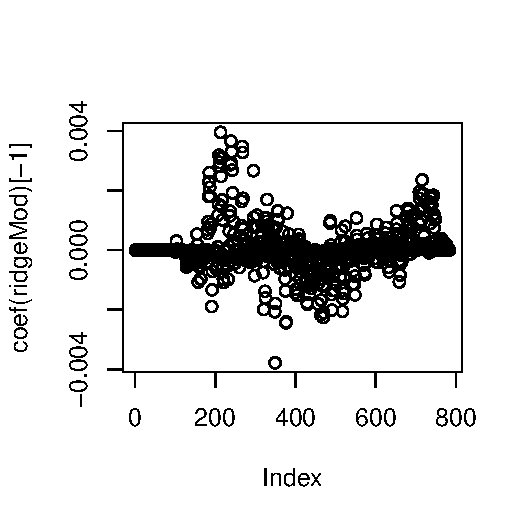
\includegraphics{Task1_files/figure-latex/plot-1} 

}

\caption{Coefficients plot}\label{fig:plot}
\end{figure}

It seems clear in Figure 2. how the central pixels tend to have bigger
coefficients than the first ones. This is because of the number being
drawn in the centre of the grid.

\hypertarget{predictions}{%
\subsection{Predictions}\label{predictions}}

We can now use the test set (properly transformed and filtered) in order
to make some predictions using the model and measure the performance of
the model. We are using a logistic binomial model, so the prediction is
a estimated probability of the event being a certain class. Since we
want a binomial output for computing the accuracy of the prediction, a
cut-off for the probability is needed. The selected cut-off will be the
naive \(0.5\).

\begin{Shaded}
\begin{Highlighting}[]
\CommentTok{\# Predictions}
\NormalTok{predictions }\OtherTok{\textless{}{-}} \FunctionTok{predict}\NormalTok{(ridgeMod, }\AttributeTok{type =} \StringTok{"response"}\NormalTok{,}
                       \AttributeTok{newx =} \FunctionTok{as.matrix}\NormalTok{(test}\SpecialCharTok{$}\NormalTok{px))}

\CommentTok{\# Convert predicted probabilities to class labels (4 or 9)}
\NormalTok{predicted\_classes }\OtherTok{\textless{}{-}} \FunctionTok{ifelse}\NormalTok{(predictions }\SpecialCharTok{\textgreater{}} \FloatTok{0.5}\NormalTok{, }\DecValTok{9}\NormalTok{, }\DecValTok{4}\NormalTok{)}

\CommentTok{\# Evaluate the accuracy}
\NormalTok{accuracy }\OtherTok{\textless{}{-}} \FunctionTok{mean}\NormalTok{(predicted\_classes }\SpecialCharTok{==}\NormalTok{ test}\SpecialCharTok{$}\NormalTok{digit)}
\end{Highlighting}
\end{Shaded}

So the accuracy obtained in this model is 97.9351536\(\%\) for the
\(\lambda_{1se}\).

\hypertarget{further-work}{%
\subsection{Further work}\label{further-work}}

In addition, we are asked to tackle the 45 classification problems of
one versus another digit in a similar way to the previous approach and
then report the results.

We have created the 45 necessary datasets and then using vectorization
and different \texttt{apply()} functions we have computed the models and
the global accuracy. No further explanation is given because of the
optionality of the last task. The code we run is the following (3.5h
runtime approx.) and is left here for reproducibility issues.

\begin{Shaded}
\begin{Highlighting}[]
\FunctionTok{set.seed}\NormalTok{(}\DecValTok{1234}\NormalTok{)}
\NormalTok{lev }\OtherTok{\textless{}{-}} \DecValTok{0}\SpecialCharTok{:}\DecValTok{9}
\NormalTok{datasets\_train }\OtherTok{\textless{}{-}} \FunctionTok{vector}\NormalTok{(}\StringTok{"list"}\NormalTok{, }\AttributeTok{length =} \DecValTok{45}\NormalTok{)}
\NormalTok{datasets\_test }\OtherTok{\textless{}{-}} \FunctionTok{vector}\NormalTok{(}\StringTok{"list"}\NormalTok{, }\AttributeTok{length =} \DecValTok{45}\NormalTok{)}
\NormalTok{cont }\OtherTok{\textless{}{-}} \DecValTok{1}

\CommentTok{\# Generation of the datasets}
\ControlFlowTok{for}\NormalTok{ (i }\ControlFlowTok{in}\NormalTok{ lev) \{}
  \ControlFlowTok{for}\NormalTok{ (j }\ControlFlowTok{in}\NormalTok{ lev) \{}
    \ControlFlowTok{if}\NormalTok{ (i }\SpecialCharTok{\textless{}}\NormalTok{ j) \{}
\NormalTok{      train\_l }\OtherTok{\textless{}{-}}\NormalTok{ train\_nist }\SpecialCharTok{\%\textgreater{}\%}
        \FunctionTok{filter}\NormalTok{(digit }\SpecialCharTok{\%in\%} \FunctionTok{c}\NormalTok{(i, j))}
\NormalTok{      train\_l}\SpecialCharTok{$}\NormalTok{digit }\OtherTok{\textless{}{-}} \FunctionTok{droplevels}\NormalTok{(train\_l}\SpecialCharTok{$}\NormalTok{digit)}
      
\NormalTok{      test\_l }\OtherTok{\textless{}{-}}\NormalTok{ test\_nist }\SpecialCharTok{\%\textgreater{}\%}
        \FunctionTok{filter}\NormalTok{(digit }\SpecialCharTok{\%in\%} \FunctionTok{c}\NormalTok{(i, j))}
\NormalTok{      test\_l}\SpecialCharTok{$}\NormalTok{digit }\OtherTok{\textless{}{-}} \FunctionTok{droplevels}\NormalTok{(test\_l}\SpecialCharTok{$}\NormalTok{digit)}
      
      \FunctionTok{print}\NormalTok{(cont)}
\NormalTok{      datasets\_train[[cont]] }\OtherTok{\textless{}{-}}\NormalTok{ train\_l}
\NormalTok{      datasets\_test[[cont]] }\OtherTok{\textless{}{-}}\NormalTok{ test\_l}
      
\NormalTok{      cont }\OtherTok{\textless{}{-}}\NormalTok{ cont }\SpecialCharTok{+} \DecValTok{1}
\NormalTok{    \}}
\NormalTok{  \}}
\NormalTok{\}}

\CommentTok{\# Vectorized generation of the models}
\NormalTok{models }\OtherTok{\textless{}{-}} \FunctionTok{lapply}\NormalTok{(datasets\_train, }\ControlFlowTok{function}\NormalTok{(data) \{}
\NormalTok{  x }\OtherTok{\textless{}{-}} \FunctionTok{as.matrix}\NormalTok{(data[, }\DecValTok{3}\NormalTok{])}
\NormalTok{  y }\OtherTok{\textless{}{-}}\NormalTok{ data[, }\DecValTok{1}\NormalTok{]}
  \FunctionTok{cv.glmnet}\NormalTok{(}
\NormalTok{    x,}
\NormalTok{    y,}
    \AttributeTok{alpha =} \DecValTok{0}\NormalTok{,}
    \AttributeTok{standardize =} \ConstantTok{FALSE}\NormalTok{,}
    \AttributeTok{family =} \StringTok{"binomial"}\NormalTok{,}
    \AttributeTok{nfolds =} \DecValTok{10}
\NormalTok{  )}
\NormalTok{\})}

\CommentTok{\# Vectorized predictions}
\NormalTok{predictions }\OtherTok{\textless{}{-}} \FunctionTok{mapply}\NormalTok{(}\ControlFlowTok{function}\NormalTok{(model, new\_data) \{}
\NormalTok{  x\_new }\OtherTok{\textless{}{-}} \FunctionTok{as.matrix}\NormalTok{(new\_data}\SpecialCharTok{$}\NormalTok{px)}
  \FunctionTok{predict}\NormalTok{(model,}
          \AttributeTok{newx =}\NormalTok{ x\_new,}
          \AttributeTok{s =} \StringTok{"lambda.1se"}\NormalTok{,}
          \AttributeTok{type =} \StringTok{"response"}\NormalTok{)}
\NormalTok{\}, models, datasets\_test)}


\CommentTok{\# Vectorized class predictions and accuracy calculation}
\NormalTok{accuracy }\OtherTok{\textless{}{-}} \FunctionTok{mapply}\NormalTok{(}\ControlFlowTok{function}\NormalTok{(pred, mytest) \{}
\NormalTok{  y\_test }\OtherTok{\textless{}{-}} \FunctionTok{as.vector}\NormalTok{(}\FunctionTok{model.matrix}\NormalTok{(}\SpecialCharTok{\textasciitilde{}} \FunctionTok{factor}\NormalTok{(mytest}\SpecialCharTok{$}\NormalTok{digit))[, }\DecValTok{2}\NormalTok{])}
\NormalTok{  class\_predictions }\OtherTok{\textless{}{-}} \FunctionTok{ifelse}\NormalTok{(pred }\SpecialCharTok{\textgreater{}} \FloatTok{0.5}\NormalTok{, }\DecValTok{1}\NormalTok{, }\DecValTok{0}\NormalTok{)}
  \FunctionTok{mean}\NormalTok{(class\_predictions }\SpecialCharTok{==}\NormalTok{ y\_test)}
\NormalTok{\}, predictions, datasets\_test)}
\end{Highlighting}
\end{Shaded}

\begin{Shaded}
\begin{Highlighting}[]
\CommentTok{\# Generation of the table}
\NormalTok{matrix\_triang }\OtherTok{\textless{}{-}} \FunctionTok{matrix}\NormalTok{(}\DecValTok{0}\NormalTok{, }\AttributeTok{nrow =} \DecValTok{10}\NormalTok{, }\AttributeTok{ncol =} \DecValTok{10}\NormalTok{)}
\NormalTok{matrix\_triang[}\FunctionTok{upper.tri}\NormalTok{(matrix\_triang)] }\OtherTok{\textless{}{-}}\NormalTok{ accuracy}
\FunctionTok{rownames}\NormalTok{(matrix\_triang) }\OtherTok{\textless{}{-}} \FunctionTok{colnames}\NormalTok{(matrix\_triang) }\OtherTok{\textless{}{-}} \DecValTok{0}\SpecialCharTok{:}\DecValTok{9}

\FunctionTok{print}\NormalTok{(matrix\_triang)}
\end{Highlighting}
\end{Shaded}

\begin{longtable}[]{@{}
  >{\raggedright\arraybackslash}p{(\columnwidth - 20\tabcolsep) * \real{0.0909}}
  >{\raggedright\arraybackslash}p{(\columnwidth - 20\tabcolsep) * \real{0.0909}}
  >{\raggedleft\arraybackslash}p{(\columnwidth - 20\tabcolsep) * \real{0.0909}}
  >{\raggedleft\arraybackslash}p{(\columnwidth - 20\tabcolsep) * \real{0.0909}}
  >{\raggedleft\arraybackslash}p{(\columnwidth - 20\tabcolsep) * \real{0.0909}}
  >{\raggedleft\arraybackslash}p{(\columnwidth - 20\tabcolsep) * \real{0.0909}}
  >{\raggedleft\arraybackslash}p{(\columnwidth - 20\tabcolsep) * \real{0.0909}}
  >{\raggedleft\arraybackslash}p{(\columnwidth - 20\tabcolsep) * \real{0.0909}}
  >{\raggedleft\arraybackslash}p{(\columnwidth - 20\tabcolsep) * \real{0.0909}}
  >{\raggedleft\arraybackslash}p{(\columnwidth - 20\tabcolsep) * \real{0.0909}}
  >{\raggedleft\arraybackslash}p{(\columnwidth - 20\tabcolsep) * \real{0.0909}}@{}}
\toprule\noalign{}
\begin{minipage}[b]{\linewidth}\raggedright
\end{minipage} & \begin{minipage}[b]{\linewidth}\raggedright
1
\end{minipage} & \begin{minipage}[b]{\linewidth}\raggedleft
2
\end{minipage} & \begin{minipage}[b]{\linewidth}\raggedleft
3
\end{minipage} & \begin{minipage}[b]{\linewidth}\raggedleft
4
\end{minipage} & \begin{minipage}[b]{\linewidth}\raggedleft
5
\end{minipage} & \begin{minipage}[b]{\linewidth}\raggedleft
6
\end{minipage} & \begin{minipage}[b]{\linewidth}\raggedleft
7
\end{minipage} & \begin{minipage}[b]{\linewidth}\raggedleft
8
\end{minipage} & \begin{minipage}[b]{\linewidth}\raggedleft
9
\end{minipage} & \begin{minipage}[b]{\linewidth}\raggedleft
\end{minipage} \\
\midrule\noalign{}
\endhead
\bottomrule\noalign{}
\endlastfoot
0 & 0.9993876 & 0.9920558 & 0.9973571 & 0.9974579 & 0.9972532 &
0.9892221 & 0.9929215 & 0.9706697 & 0.9970850 & \\
1 & & 0.9936174 & 0.9894537 & 0.9931328 & 0.9982650 & 0.9982644 &
0.9812852 & 0.9904495 & 0.9761231 & \\
2 & & & 0.9934662 & 0.9957039 & 0.9973641 & 0.9770561 & 0.9892869 &
0.9942775 & 0.9906977 & \\
3 & & & & 0.9976759 & 0.9992197 & 0.9889558 & 0.9972016 & 0.9944351 &
0.9996759 & \\
4 & & & & & 0.9977204 & 0.9861549 & 0.9734711 & 0.9937725 & 0.9934913
& \\
5 & & & & & & 0.9897419 & 0.9978838 & 0.9935854 & 0.9979757 & \\
6 & & & & & & & 0.9923990 & 0.9793515 & 0.9943219 & \\
7 & & & & & & & & 0.9881625 & 0.9778689 & \\
8 & & & & & & & & & 0.9893617 & \\
\end{longtable}

Note how the previous code takes the base factor as de smallest digit.
This makes sense since the datasets are created that way and also
\texttt{class\_prediction} loop is working the same way.

\hypertarget{references}{%
\subsection*{References}\label{references}}
\addcontentsline{toc}{subsection}{References}

\hypertarget{refs}{}
\begin{CSLReferences}{1}{0}
\leavevmode\vadjust pre{\hypertarget{ref-Garcia-Portugues2023}{}}%
García-Portugués, E. 2023. \emph{Notes for Predictive Modeling}.
\url{https://bookdown.org/egarpor/PM-UC3M/}.

\leavevmode\vadjust pre{\hypertarget{ref-glmnet}{}}%
Tay, J. Kenneth, Balasubramanian Narasimhan, and Trevor Hastie. 2023.
{``Elastic Net Regularization Paths for All Generalized Linear
Models.''} \emph{Journal of Statistical Software} 106 (1): 1--31.
\url{https://doi.org/10.18637/jss.v106.i01}.

\leavevmode\vadjust pre{\hypertarget{ref-dplyr}{}}%
Wickham, Hadley, Romain François, Lionel Henry, Kirill Müller, and Davis
Vaughan. 2023. \emph{Dplyr: A Grammar of Data Manipulation}.
\url{https://CRAN.R-project.org/package=dplyr}.

\leavevmode\vadjust pre{\hypertarget{ref-enwiki:1199732782}{}}%
Wikipedia contributors. 2024. {``MNIST Database --- {Wikipedia}{,} the
Free Encyclopedia.''}
\url{https://en.wikipedia.org/w/index.php?title=MNIST_database\&oldid=1199732782}.

\end{CSLReferences}

\end{document}
